\documentclass{ctexart}
\usepackage[left=1.5cm,right=1.5cm,top=1.5cm,bottom=1.5cm]{geometry}
\usepackage{listings}
\usepackage[dvipsnames]{xcolor}
\usepackage{cite}
\usepackage{diagbox}
\usepackage{fancyhdr} % 加载fancyhdr宏包,用于设置页眉和页脚
\pagestyle{fancy} % 设置页面样式
\fancyhf{} % 清除默认的页眉和页脚的内容
\fancyfoot[C]{\thepage} 
\renewcommand{\headrulewidth}{0pt} % 将页眉的横线宽度设置为0pt

\usepackage{graphicx}
\usepackage{longtable}
\usepackage{tabularx}
\usepackage{float}
\usepackage{amsmath}%引用宏包要放在documentclass后面,否则报错
\usepackage{hyperref}
\usepackage{bm}
\usepackage{amssymb}
\usepackage{esint}
\usepackage{booktabs}
%\usepackage{subfiles}%用于分章节管理引用,使各章节引用来源于各自的文件,编号相互独立
\usepackage{amsthm}
\title{电子工艺实践课程报告}
\author{Leo}
\date{\today}
\begin{document}
\maketitle



\section{实验目的}
\begin{enumerate}
    \item 识别和使用常用电子元器件,掌握常用电子仪器、仪表的使用方法;
    \item 熟悉电子产品的设计和生产过程;
    \item 学习 multisim 仿真软件的使用方法;
    \item 掌握用 Altium Designer 软件设计原理图和印制电路板图;
    \item 掌握电路的焊接、安装、检查及调试方法.
\end{enumerate}
\section{实验原理}
\subsection{流水灯电路工作原理分析}
本课程要求完成一个含有4个LED灯的流水灯电路,每个时钟下有三个灯亮,亮灯的流动方向要一致。设四个灯为A,B,C,D.则流水灯的状态转移可以写成:1110-0111-1011-1101-1110.若规定亮灯的移动方向为右移,则利用移位寄存器74194可以写出SR的表达式
\begin{equation}
    SR=\overline{Q_A Q_B Q_C}
\end{equation}
检查自启动,做出状态转移图如图\ref{状态转移图},可以发现经过有限个时钟,该电路可以回到主循环上。
\begin{figure}[H]
    \centering
    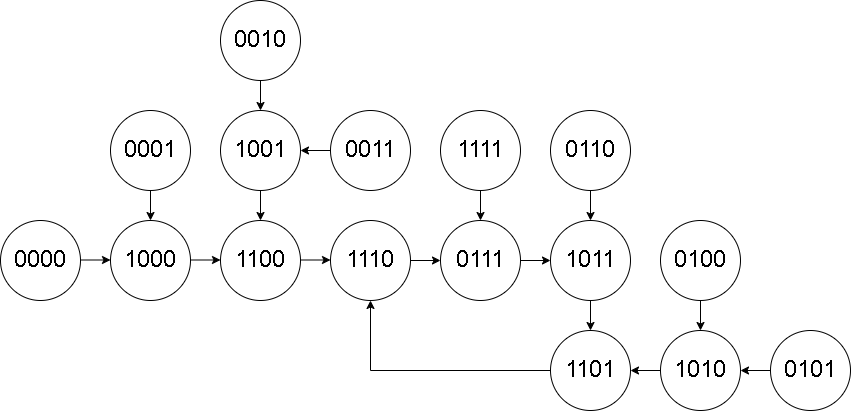
\includegraphics[scale=0.5]{pic/状态转移图.drawio.png}
    \caption{状态转换图}
    \label{状态转移图}
\end{figure}
\subsection{Altium Designer绘图}
\subsubsection{绘制原理图}
使用Multisim仿真验证合理性后,在Altium Designer中绘制原理图。首先新建项目,在项目中新建Schematic,出现一份空白的.SchDoc文件,在该文件中仿照Multisim连线。需要注意的有以下几点
\begin{enumerate}
    \item 要注意芯片的型号,尤其是封装方式
    \item 设置元件流水号最好使用默认设置
    \item 元件之间连线时要看清是否真的连上
    \item 部分芯片没有自动展示其接地和高电平引脚,需要手动调出来。具体操作为:右击元件,在下拉栏里找到Properties->graphical->选择“Show all pins on sheet”
\end{enumerate}
\subsubsection{绘制印制电路板图}
使用PCB向导创建PCBDoc文件,载入网络表文件,这样就会出现在原理图中的所有元件,并显示引脚之间的连接关系,便于后续引导手动布线。
\subsubsection{注意事项}
\begin{enumerate}
    \item VCC和GND从PLUG引出的第一根线需要加粗(至100mil),为的是提高电流的流量。其他共电源或共地的线不用加粗。具体的设置方法为:用正常的线径连线后,通过上方菜单栏的Design->Rules->将Routing-Constraints中的Max width设置为100mil,保存后退出,在想要加粗的线上右击,在Properties中改变线径即可。
    \item 画线之前要选中正确的层。Bottom层是蓝色线,Top层是红色线(飞线)
    \item 画线之前,要将载有元件的托盘删除,并删除pcb版周围的红线
    \item 任何时候出现绿色的线,表示这条线有问题,需要删除重画
\end{enumerate}
走线规范
\begin{enumerate}
    \item 芯片朝向应一致;元件摆放要整齐
    \item 走线时转弯角度不能小于90度
    \item 走线尽量不在芯片内部。由于万能板的限制,芯片内的平行线不能超过两根
    \item 时钟信号源、电源和地线的接口尽量放在板子的边缘
    \item 地线尽量走板子的四周边沿
    \item 走线尽量短而均匀,线与线之间间隔适当
    \item 尽量不飞线
\end{enumerate}
\subsection{焊接工艺及注意事项}
本次焊接使用万能板,采用堆焊工艺。只能根据洞的分布来布线,所以无法做到以钝角转弯。
焊接流程为
\begin{enumerate}
    \item 大致摆放元件位置,设计走线方法,做到焊接前心中有数
    \item 从高度较低的元件(如电阻)开始焊接,最后焊较高的元件(比如芯片)
    \item 芯片底座要先插入芯片再焊到板子上,避免因为焊接误差导致芯片无法插入底座
    \item 先把元件全部焊到板子上再连线
    \item 最后处理飞线和边缘的接口
\end{enumerate}
焊接时应注意以下几点
\begin{enumerate}
    \item 堆焊要足够多,防止虚焊
    \item 同一个地方加热不能太久,如果要改,应先待其冷却后再来
    \item 元件焊好之后应将其在背面的引脚处理干净
    \item 焊接温度不宜过高
\end{enumerate}
\section{实验内容}
\subsection{软件绘制的原理图及PCB图}
在Altium Designer中绘制的原理图如图\ref{altium原理图}所示
\begin{figure}[H]
    \centering
    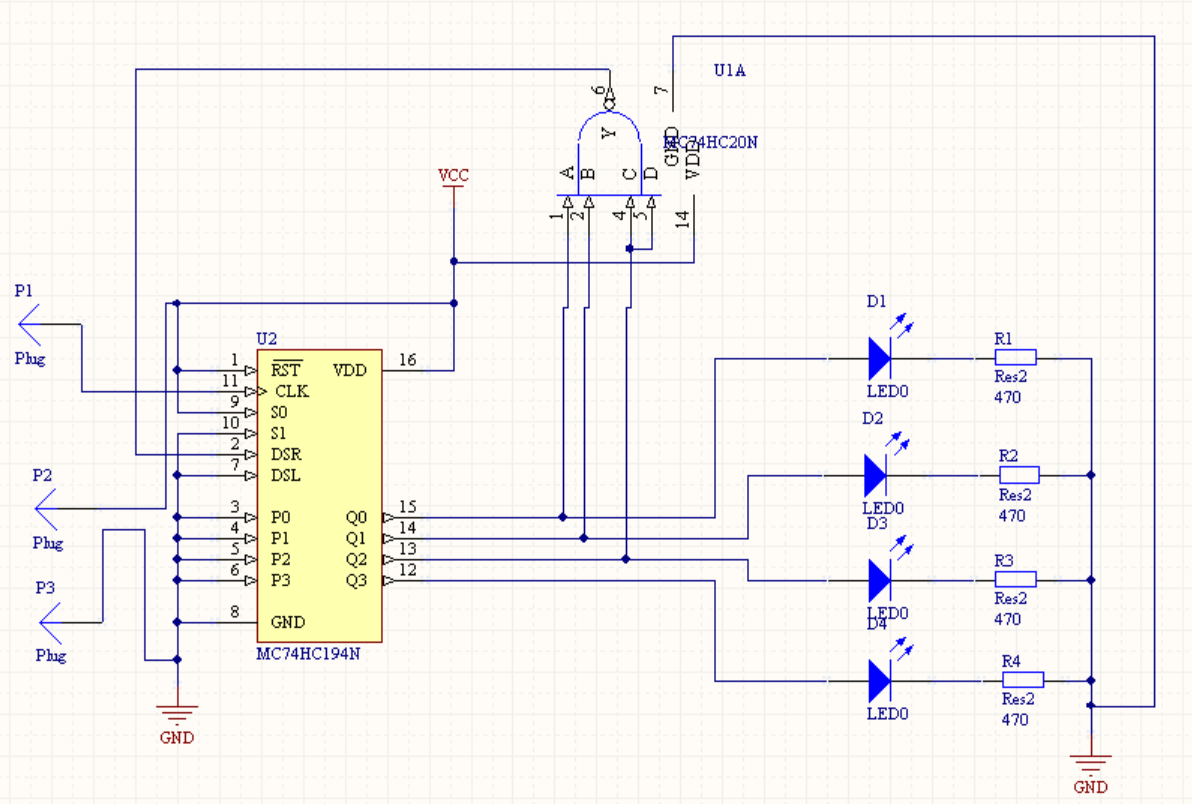
\includegraphics[scale=0.7]{pic/altium原理图.png}
    \caption{Altium 原理图}
    \label{altium原理图}
\end{figure}
图中所示的原理同经过软件检查无误,可以进入PCB版图的绘制。

在Altium Designer中绘制的PCB图如图\ref{altiumPCB图}所示
\begin{figure}
    \centering
    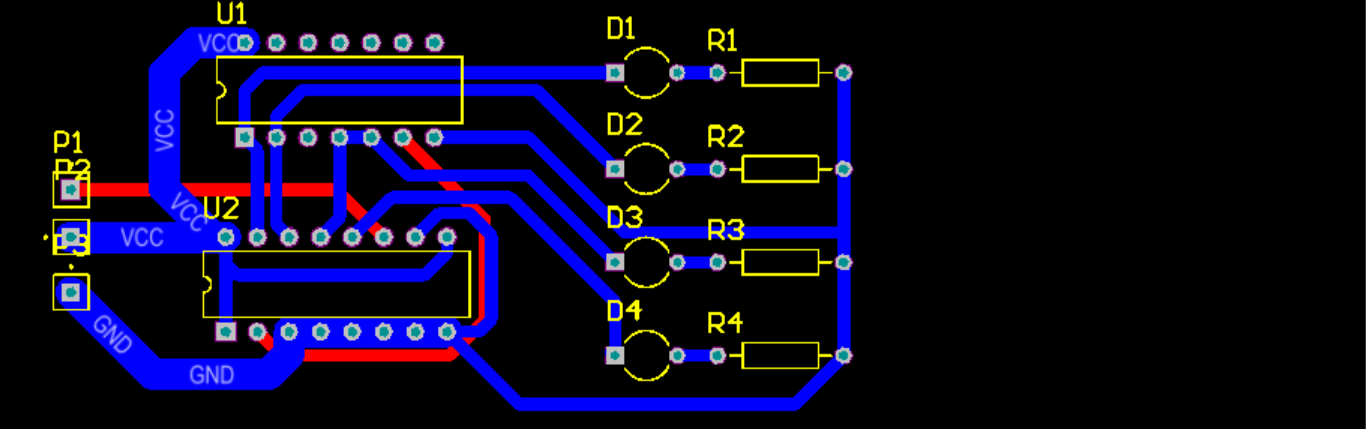
\includegraphics[scale=0.7]{pic/altiumPCB图.png}
    \caption{Altium PCB图}
    \label{altiumPCB图}
\end{figure}
\subsection{装配焊接电路过程}
如图\ref{焊接过程}是刚焊接完元件时的照片
\begin{figure}[H]
    \centering
    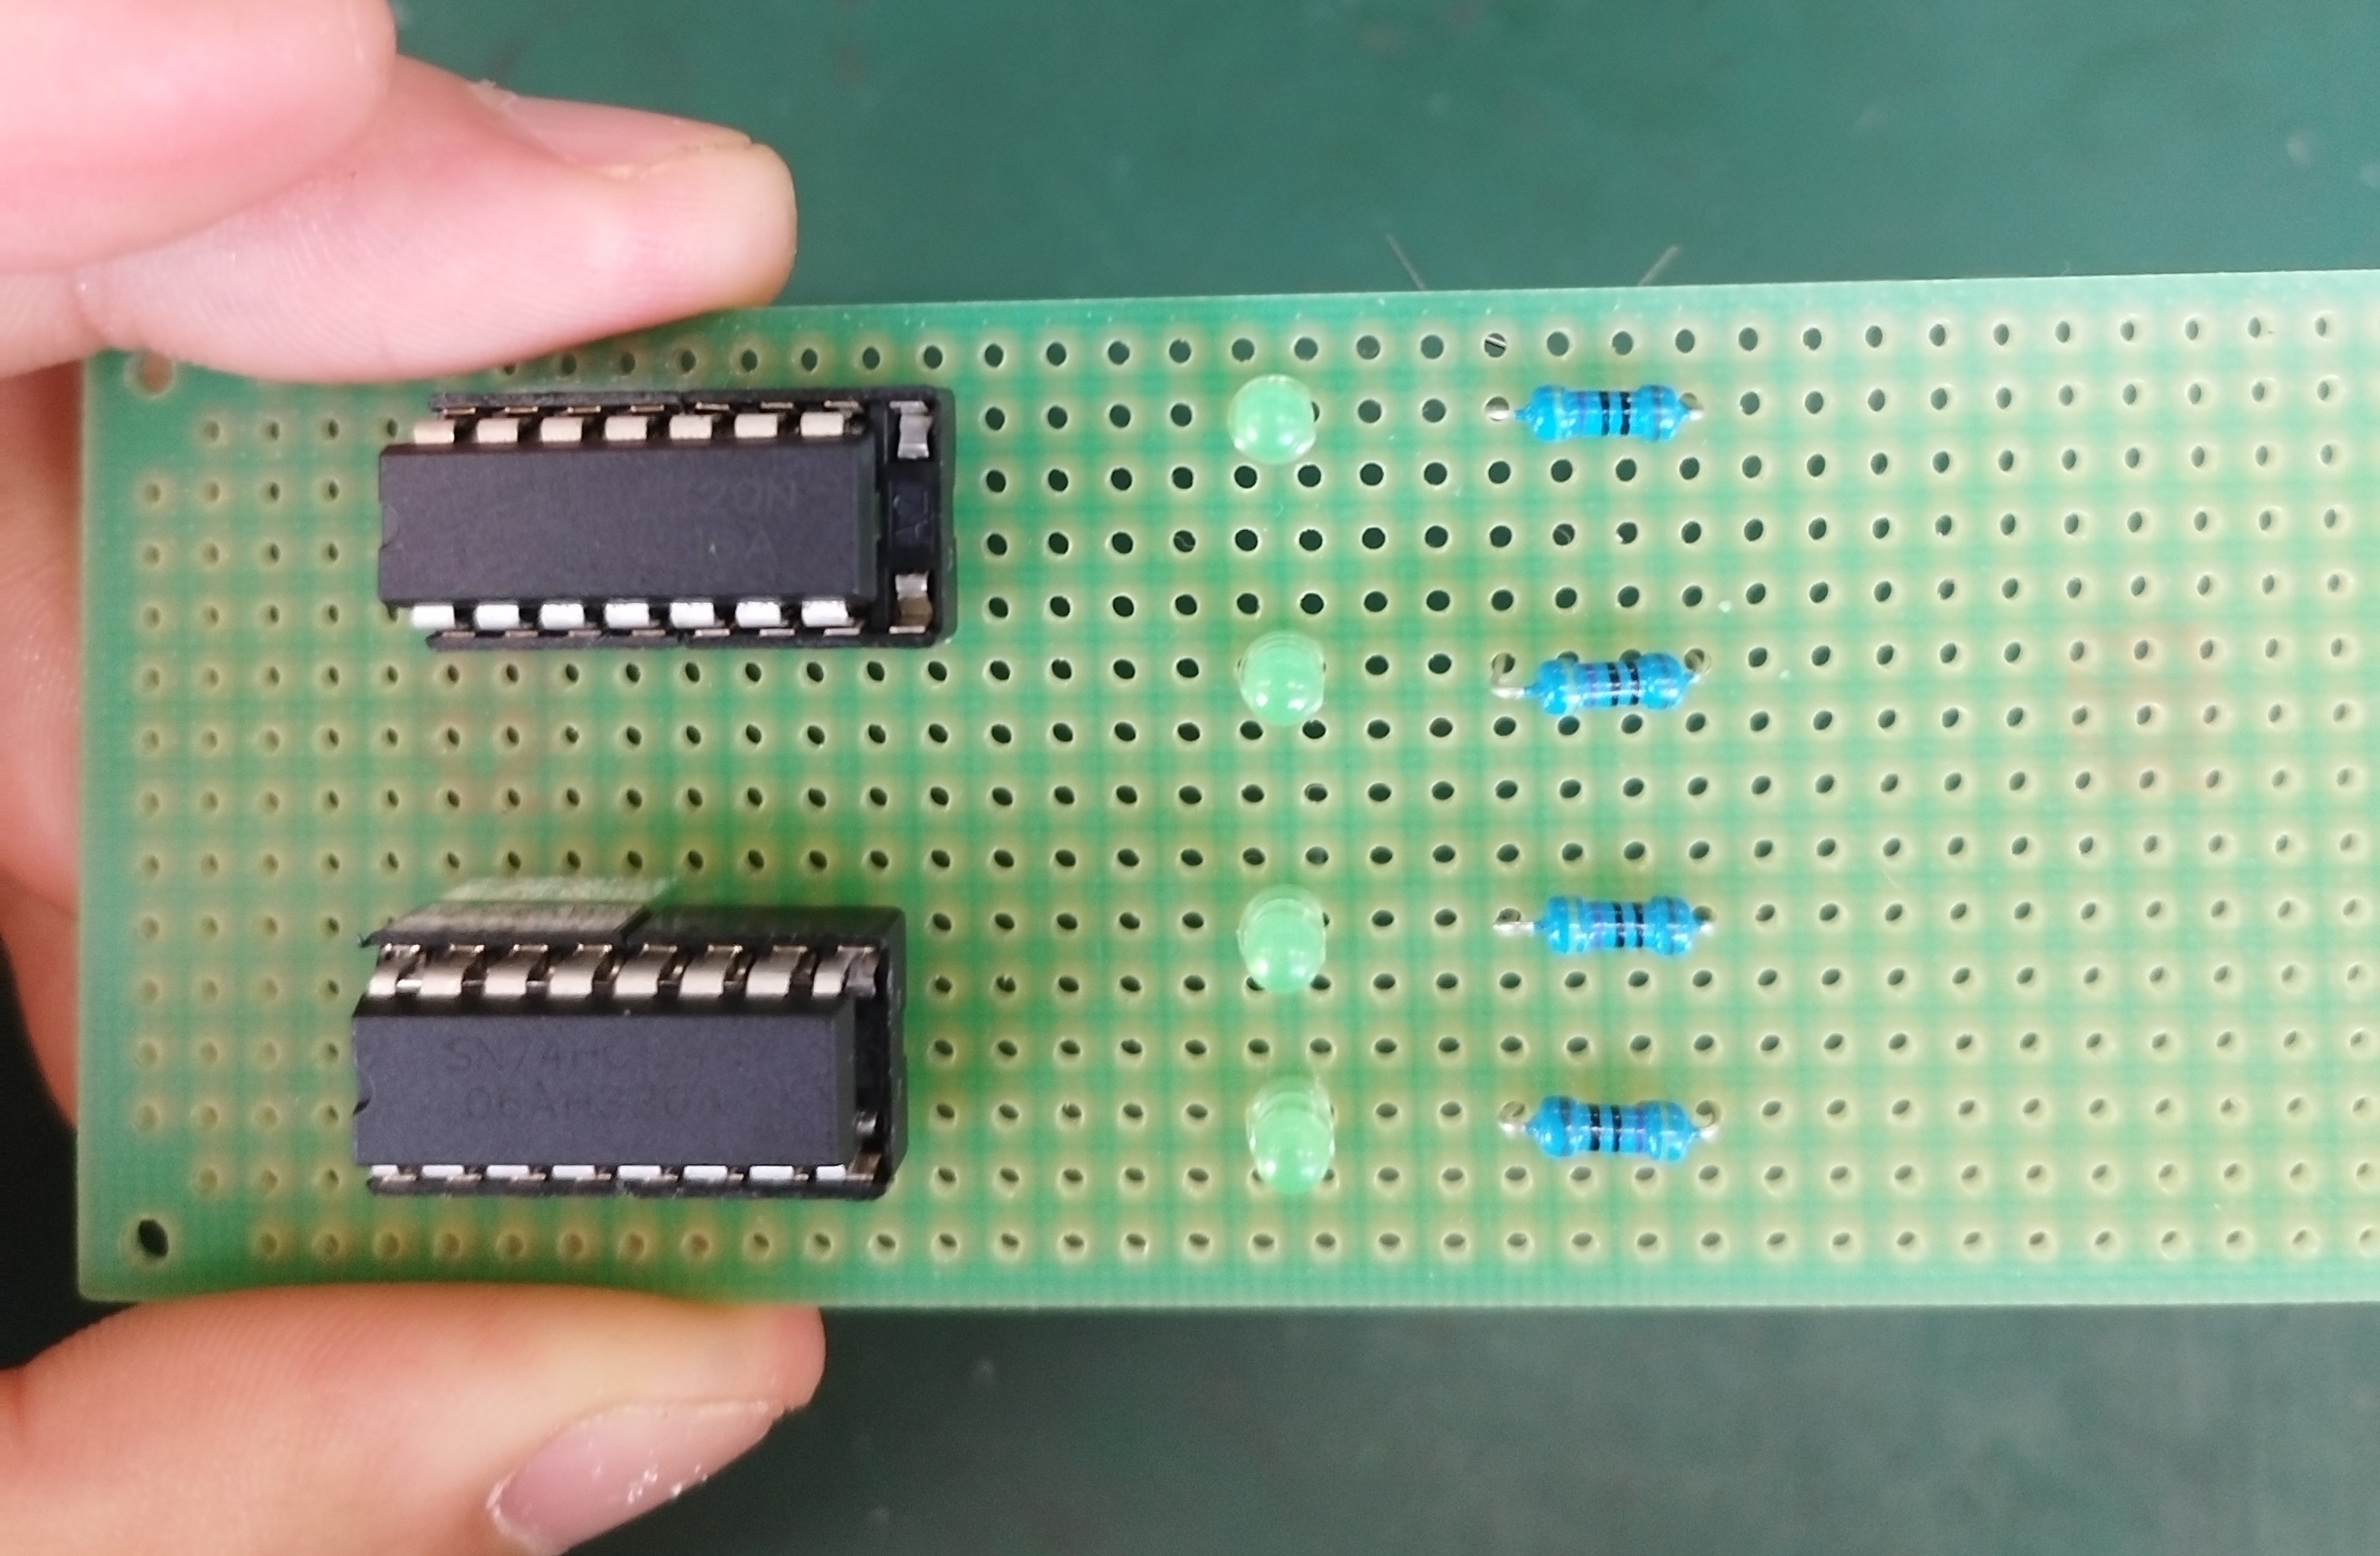
\includegraphics[scale=0.1]{pic/焊接过程.jpg}
    \caption{焊接过程}
    \label{焊接过程}
\end{figure}
\subsection{万能板上制作的电路,正面、反面实物图}
\begin{figure}[H]
    \centering
    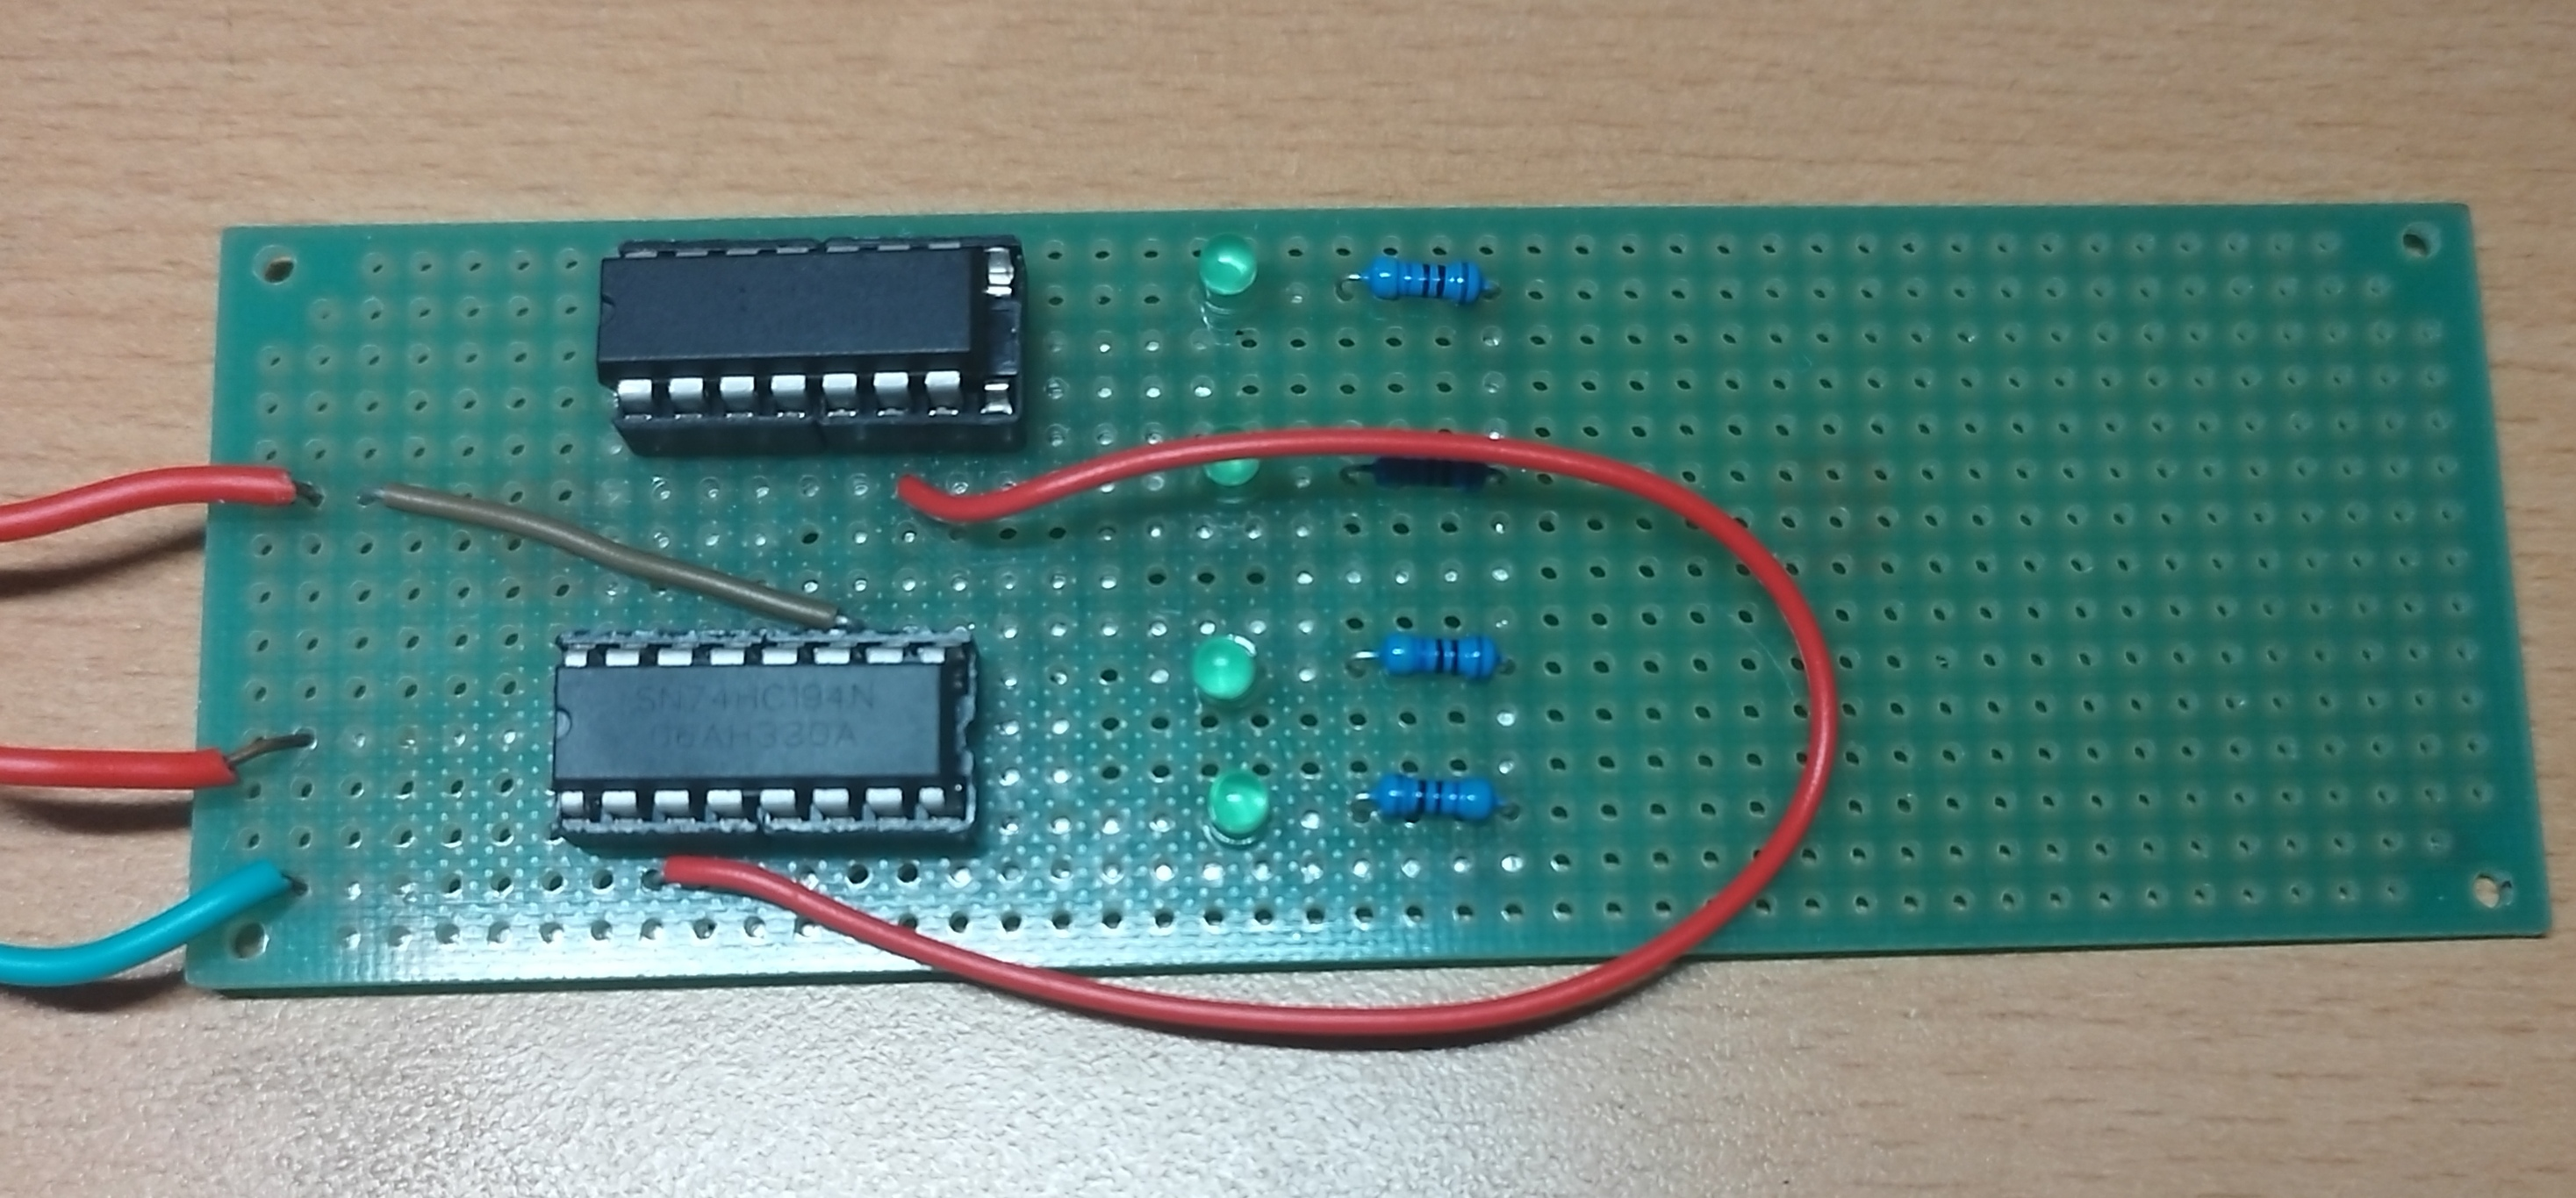
\includegraphics[scale=0.1]{pic/实物图正面.jpg}
    \caption{正面实物图}
    \label{正面}
\end{figure}
\begin{figure}[H]
    \centering
    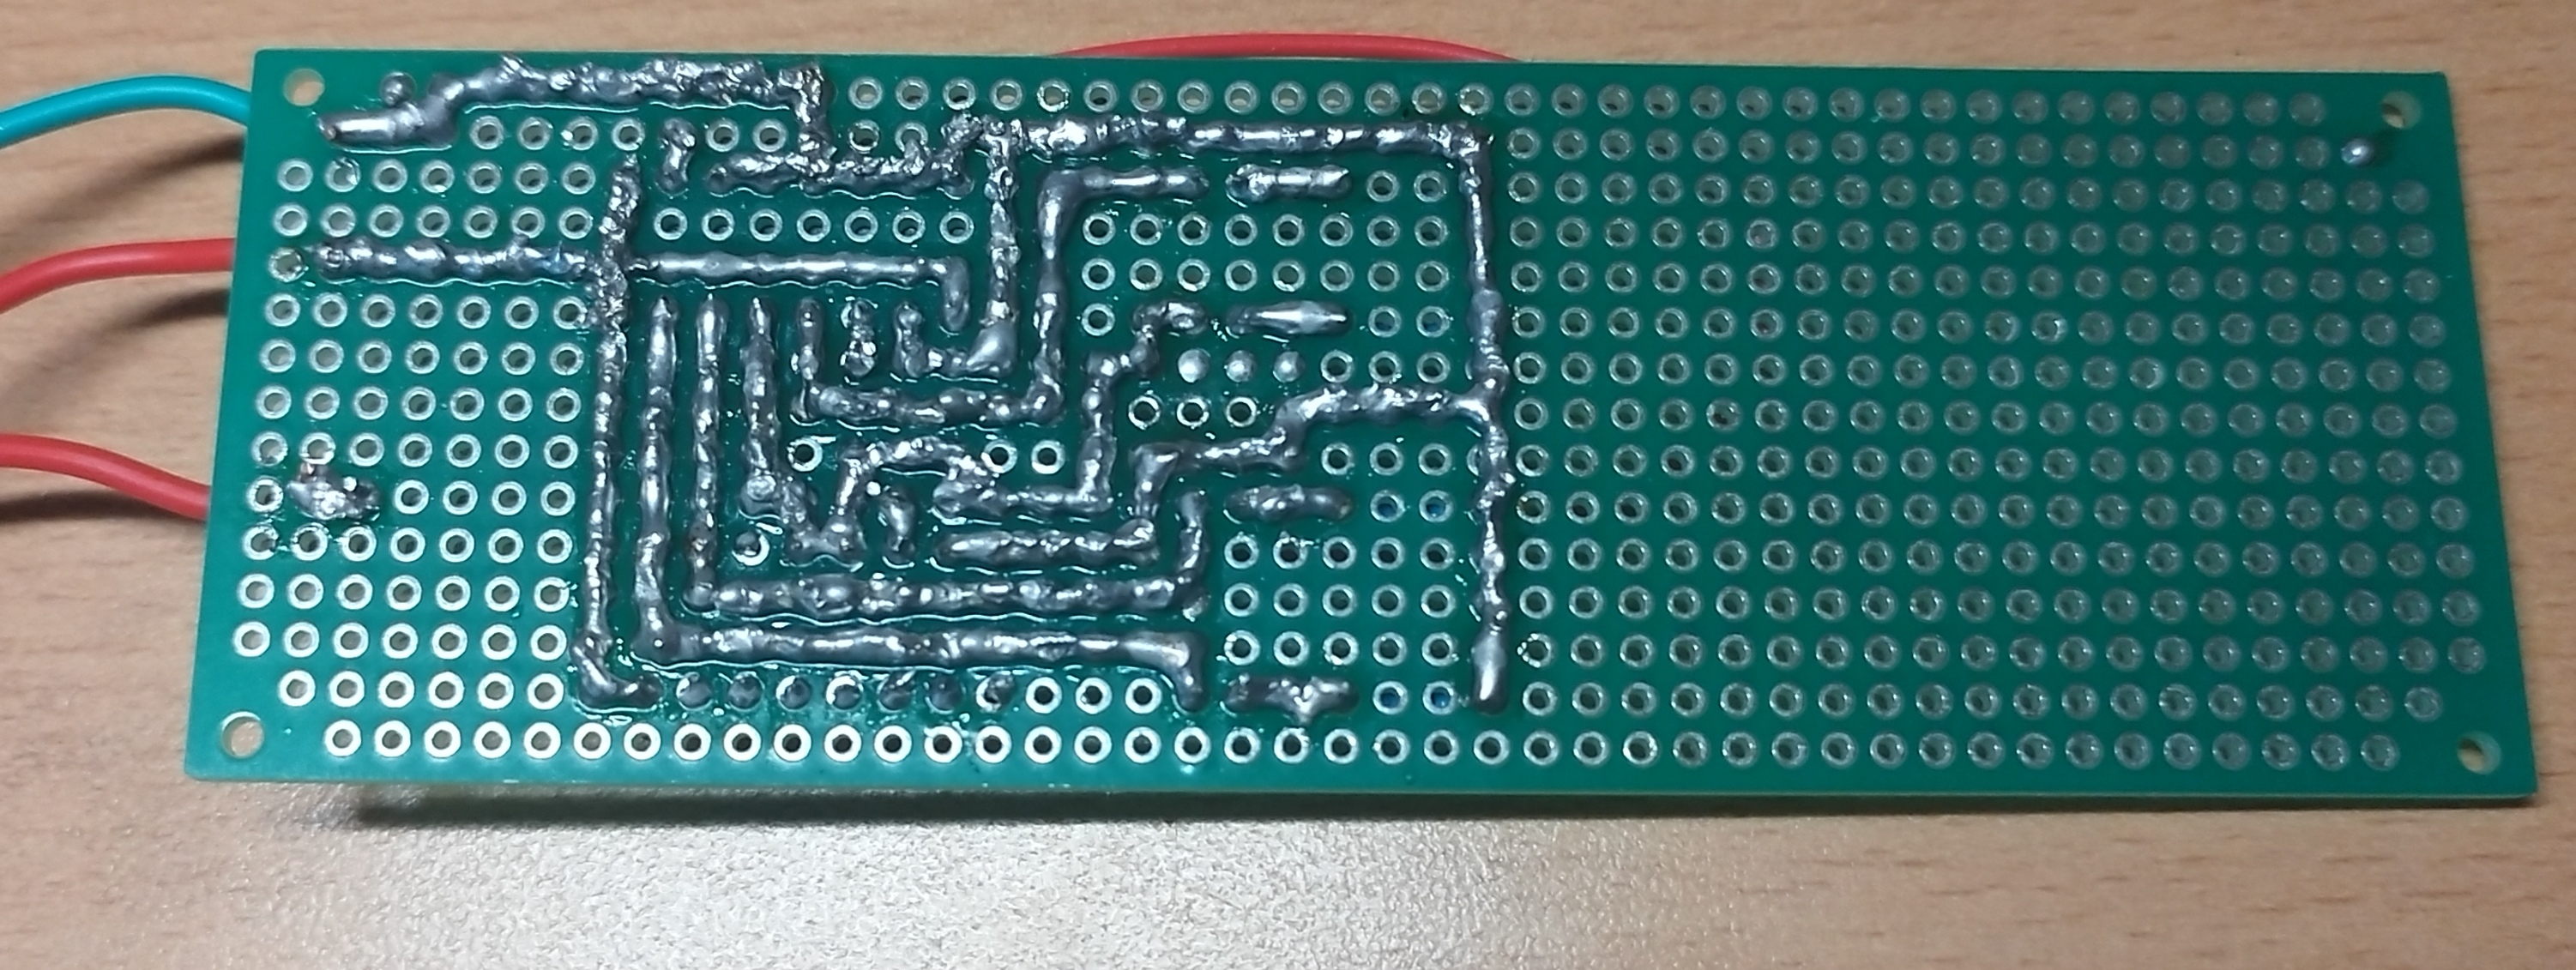
\includegraphics[scale=0.1]{pic/实物图反面.jpg}
    \caption{反面实物图}
    \label{反面}
\end{figure}
\subsection{通电测试,各级波形图及参数}
给板子通电,用新号发生器给芯片一适宜时钟频率。可以看到流水灯按设定的规律闪烁。使用示波器,分别测量时钟信号与第一个灯、第一个灯与第二个灯、第一个灯与第三个灯、第一个灯与第四个灯的波形图,如图\ref{时钟信号与第一个灯的波形图}-\ref{第一个灯与第四个灯的波形图}所示,根据相位关系也可以知道该电路实现了流水灯的功能。
\begin{figure}[H]
    \centering
    \begin{minipage}{0.45\textwidth}
    \centering
           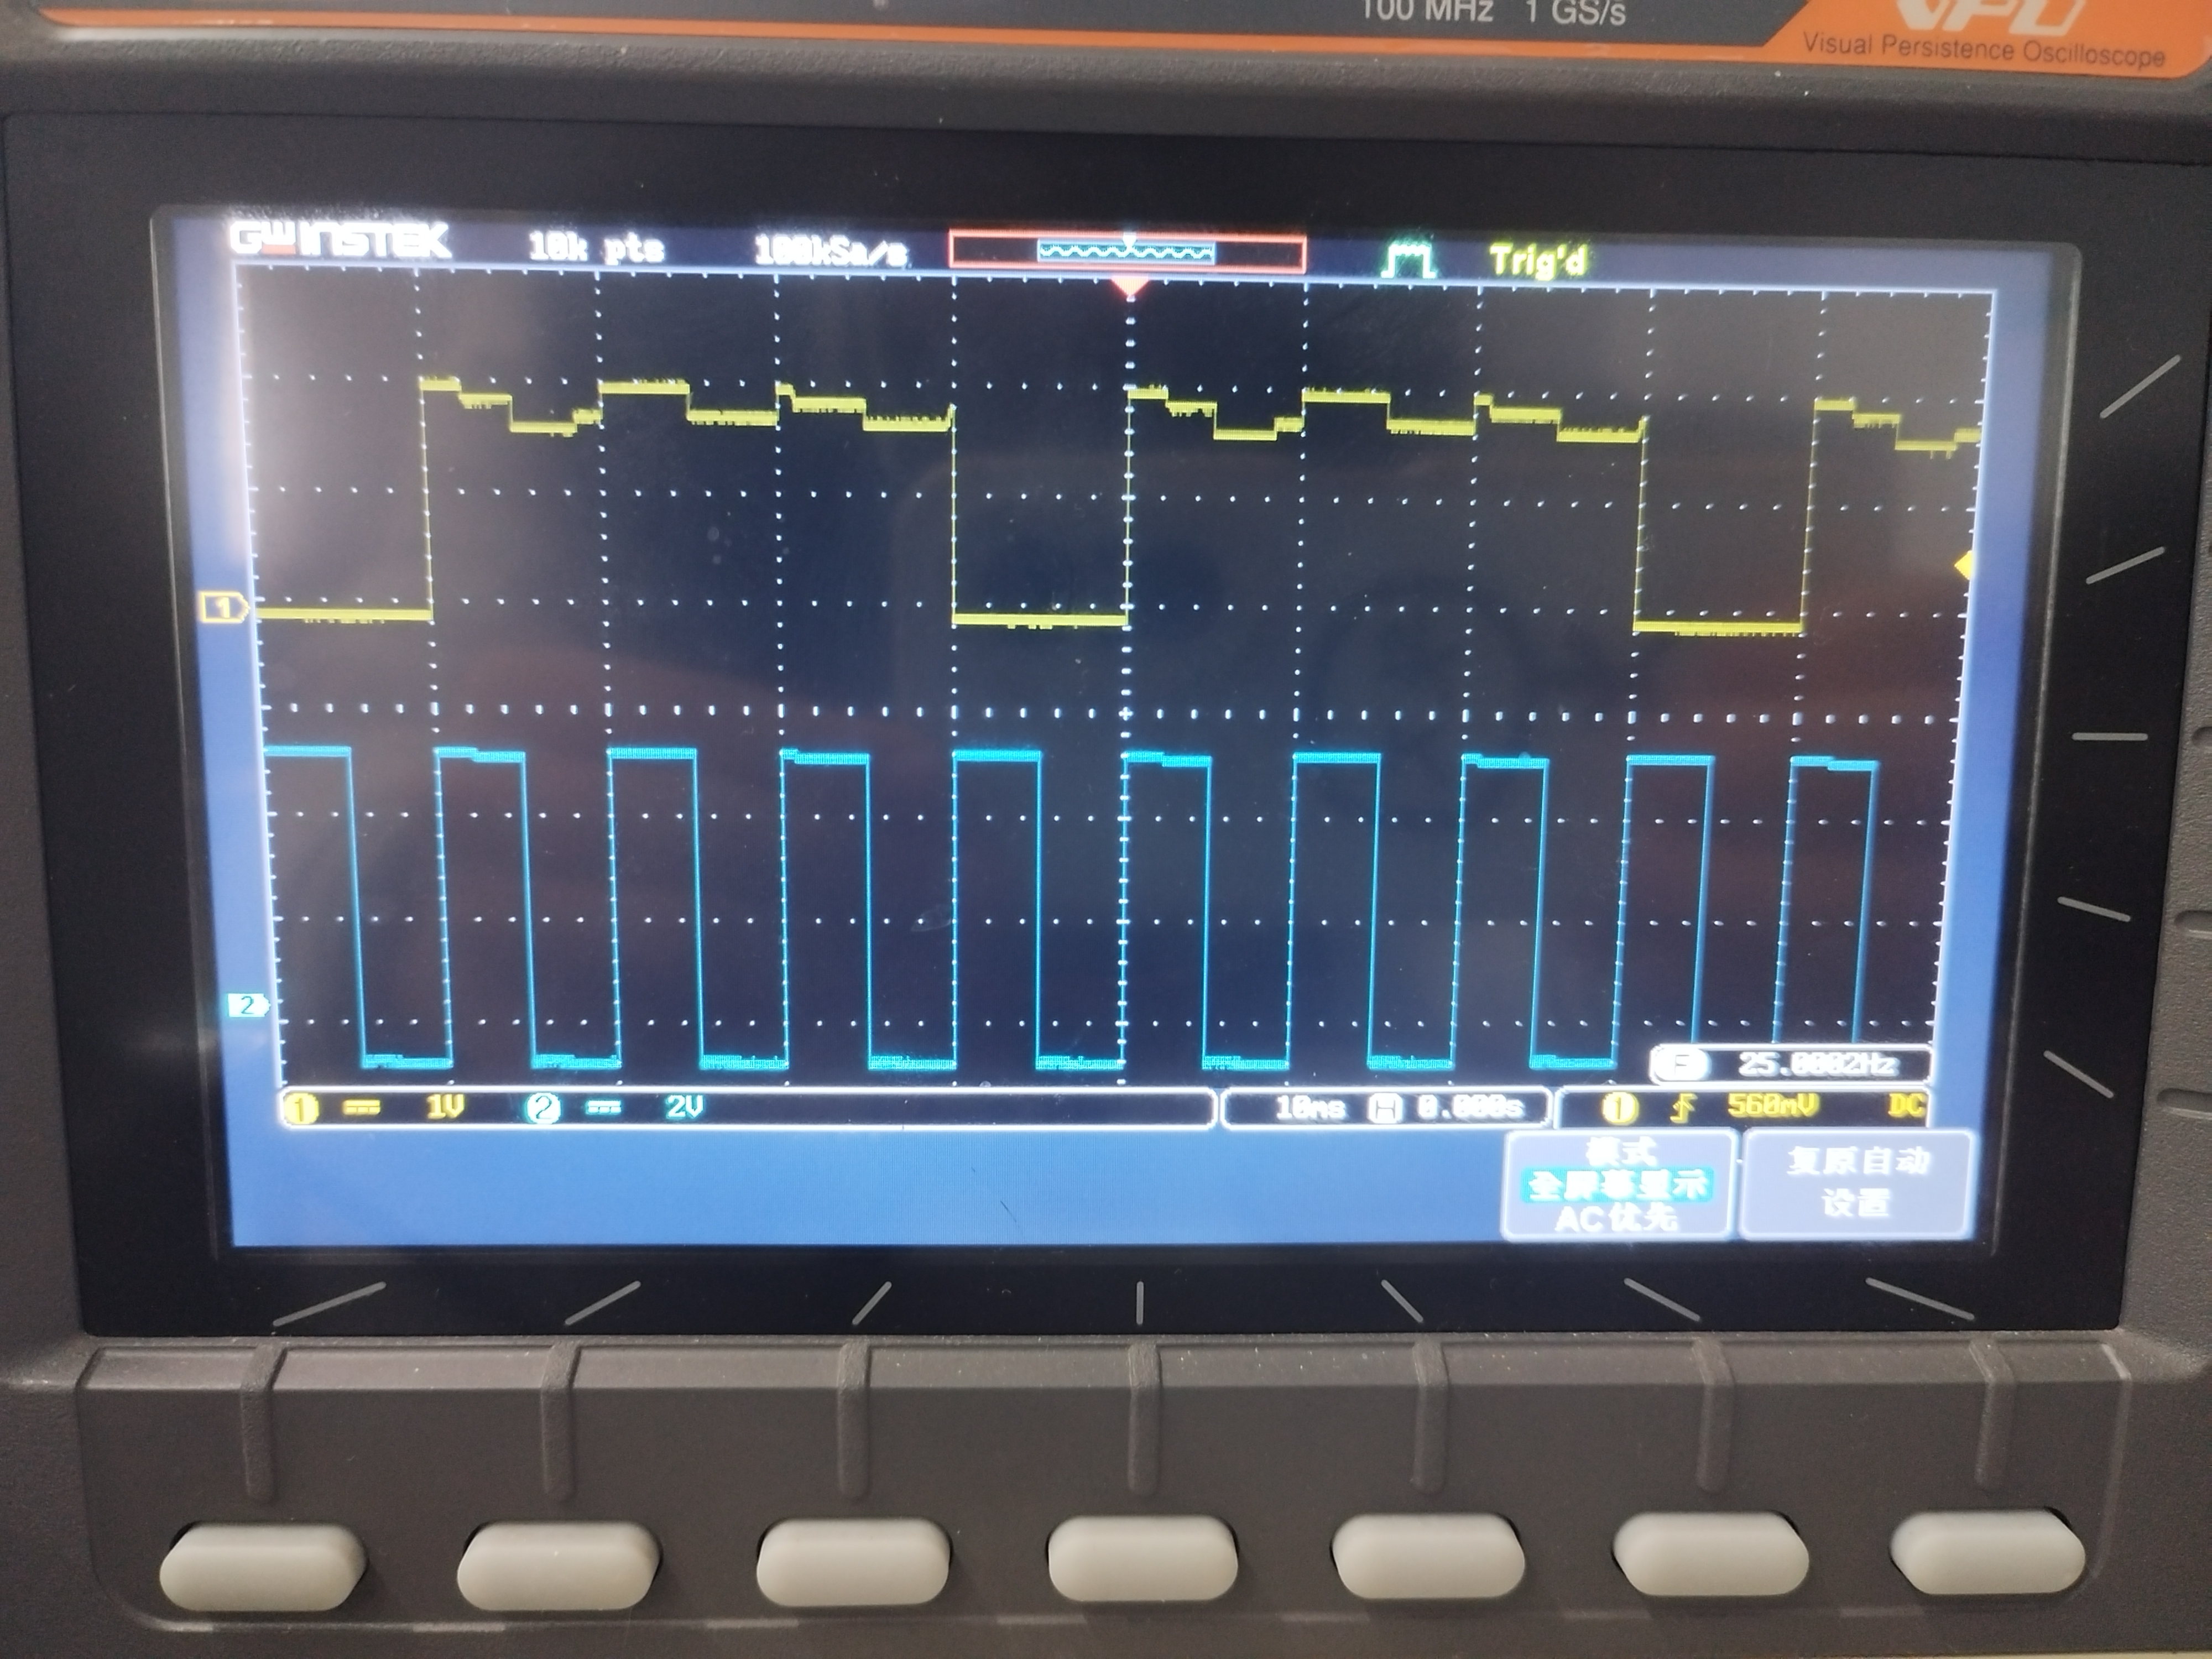
\includegraphics[width=1\textwidth]{pic/时钟与灯1.jpg}
           \caption{时钟信号与第一个灯的波形图}
    \label{时钟信号与第一个灯的波形图}
    \end{minipage}
    \hspace{0.05\textwidth}
    \begin{minipage}{0.45\textwidth}
    \centering
           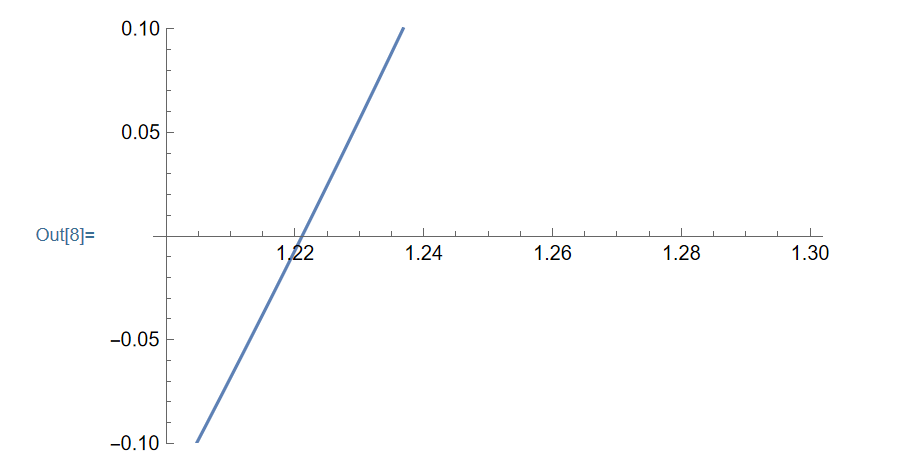
\includegraphics[width=1\textwidth]{pic/2.jpg}
           \caption{第一个灯与第二个灯的波形图}
    \label{第一个灯与第二个灯的波形图}
    \end{minipage}
\end{figure}
\begin{figure}[H]
    \centering
    \begin{minipage}{0.45\textwidth}
    \centering
           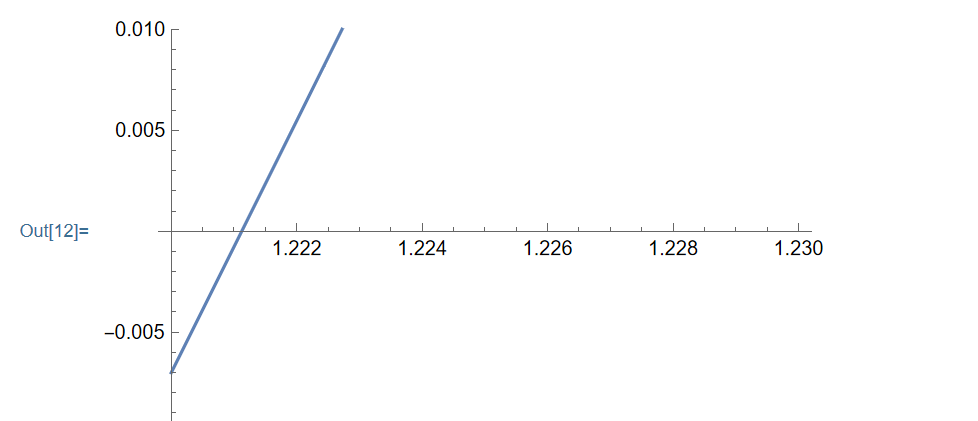
\includegraphics[width=1\textwidth]{pic/3.jpg}
           \caption{第一个灯与第三个灯的波形图}
    \label{第一个灯与第三个灯的波形图}
    \end{minipage}
    \hspace{0.05\textwidth}
    \begin{minipage}{0.45\textwidth}
    \centering
           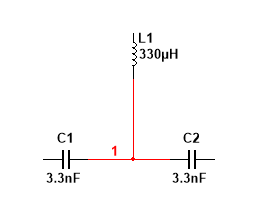
\includegraphics[width=1\textwidth]{pic/4.jpg}
           \caption{第一个灯与第四个灯的波形图}
    \label{第一个灯与第四个灯的波形图}
    \end{minipage}
\end{figure}
\subsection{通过Multisim软件仿真流水灯电路,观察仿真波形}
利用74194和7420,在Multisim中搭建仿真电路验证上述设计的合理性。如图\ref{multisim}所示
\begin{figure}[H]
    \centering
    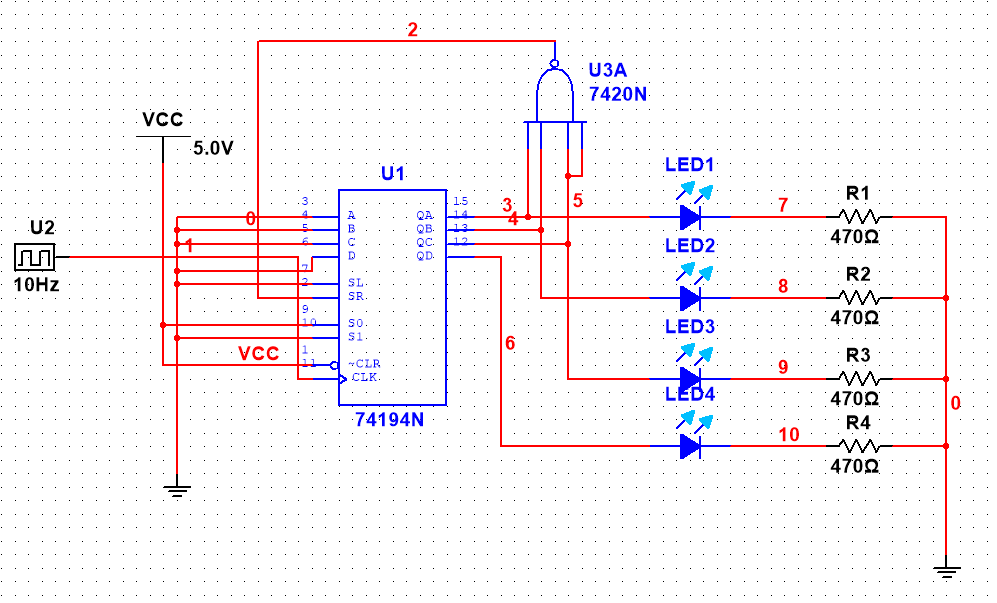
\includegraphics[scale=0.7]{pic/multisim.png}
    \caption{Multisim仿真电路图}
    \label{multisim}
\end{figure}
点击运行可以看到从上到下亮灯的循环。
\section{心得体会及建议}
\begin{enumerate}
    \item 设计PCB版图时要将线径考虑清楚。否则会出现用细线可以连接但换用粗线后空间不够的问题
    \item 堆焊时焊锡要给足,第一次焊接时就是因为焊锡不够,导致多处焊点虚焊,电路功能异常
    \item 焊接之前应充分考虑好再动手,注意预留飞线和接口的焊点,更要注意布线密集处是否有可能形成“死路”。
    \item 上电之后,通过示波器观察到灯上的高电平信号总是出现小幅度的误差,但该误差非常稳定,不像是焊接出现的问题。可能是芯片质量原因,导致电平精度仅仅能满足门限要求而与实际高电平有肉眼可见的差距。
\end{enumerate}
\end{document}